\documentclass[11pt]{article}

\setlength{\oddsidemargin}{-0.25 in}
\setlength{\evensidemargin}{-0.25 in}
\setlength{\topmargin}{-0.9 in}
\setlength{\textwidth}{7.0 in}
\setlength{\textheight}{9.0 in}
\setlength{\headsep}{0.75 in}
\setlength{\parindent}{0.3 in}
\setlength{\parskip}{0.1 in}
\usepackage{epsf}
\usepackage{pseudocode}
\usepackage{enumitem}
\usepackage{amsmath}
\usepackage{amssymb}
\usepackage{color}
\usepackage[normalem]{ulem}
\usepackage{graphicx}
\usepackage[export]{adjustbox}
\pagenumbering{arabic}
\def\O{\mathop{\smash{O}}\nolimits}
\def\o{\mathop{\smash{o}}\nolimits}
\newcommand{\e}{{\rm e}}
\newcommand{\R}{{\bf R}}
\newcommand{\Z}{{\bf Z}}

%% display solutions or not
\newif\ifsol
\soltrue % comment out to hide solutions

\usepackage[colorinlistoftodos]{todonotes}
%% todo tracker -- overleaf v2 has better one it uses but will default to this if compiled on something that doesn't have built-in todo
\newcommand{\todo}[1]{\textbf{\textcolor{red}{#1}}}

\title{Midterm 2 Review Notes}
\author{CS 182 - Artificial Intelligence}
\date{}
\begin{document}
\maketitle

\renewcommand{\labelenumii}{\arabic{enumii}.}
\setlength{\parindent}{0pt}

Note: this document is mainly a compilation of previous section notes with small extensions to better cover the testable topics. It also includes a review of Game Theory at high level and zero-sum Nash Equilibrium which are both testable. While we have tried our best to cover all testable topics please also review the lecture slides to make sure you review all of the material.

\section{Robot Motion Planning}

To make trajectory plans in robotics, we distinguish between two spaces:
\begin{itemize}
\item The {\bf{task space}} of a robot is the standard, Cartesian space in which it moves. It is usually defined by 3-dimensional (x, y, z) coordinates (but if one of the dimensions is irrelevant, such as for a Roomba, we can also define the task space by just (x, y)).
\item The {\bf{configuration space}} of a robot is the $n$-dimensional space of joint angles that fully defines the positioning of the robot. The number $n$ can be thought of as the number of degrees of freedom.
\end{itemize}

The relationship between a point in the task space and a point in the configuration space is determined by the structure and geometry of the robot. In the forward direction, {\bf{forward kinematics}} is the mapping of a robot configuration to an {\bf{end-effector}} (hand) position in task space. Conversely, {\bf{inverse kinematics}} maps a point in task space to a robot configuration. Remember, a robot in configuration space is simply a point!

Since the path-planning algorithms we discussed are based on random sampling, there are no deterministic guarantees of completeness and optimality that were discussed for search algorithms. Instead, we consider {\bf{probabilistic completeness}} and {\bf{probabilistic optimality}}, which ask whether algorithms are complete or optimal in the limit that the number of samples approaches infinity.

We then considered a handful of algorithms including:
\begin{itemize}
    \item {\bf{Rapidly-exploring Random Tree (RRT):}} This algorithm accepts a start and goal location. To build a path, it iteratively: (1) samples states $s \in S$ until it finds one that is collision-free; (2) finds closest state $s_c \in T$; (3) extends $s_c$ toward $s$; (4) adds resulting state $s’$ to $T$; (5) repeats until $T$ contains a path from $s_0$ to $s_{goal}$. This algorithm is probabilistically complete, and searches for feasbile paths. A variant includes {\bf{goal-directed sampling}}, which augments the sampling step (1). Instead of just sampling randomly, we sample the goal with a (small) probability $p$. This makes it more likely that the tree actually reaches the goal, rather than waiting until it "stumbles" into it.
    \item {\bf{Bi-directional RRT:}} This a variant on RRT which grows two trees -- one starting from the start state and one from the goal state -- and alternates between the two of them for sampling and extending. This version tends to perform better on difficult "bugtrap" problems.
    \item {\bf{RRT*:}} While RRT is very widely used, it searches for feasible but not optimal paths. RRT* is a variant on RRT that has guarantees of probabilistic optimality. The algorithm iteratively: sample state $s \in S$ until one is found that is collision-free; (2) find closest state $s_c \in T$; (3) extend $s_c$ toward $s$ resulting in state $s'$; (4) find all $s_{near} \subseteq T$ within a distance d to $s'$; (5) find $s_{min} \in s_{near}$ that has the lowest path cost to $s_0 \rightarrow s_{min} \rightarrow s'$; (6) add edge $s_{min} \rightarrow s'$ to $T$; (7) check path cost through $s'$ to all states in $s \in s_{near}$, if any are lower than existing path cost to $s$, then ``rewire'' tree to include edge $s' \rightarrow s$; (8) repeat until maximum iterations reached and $T$ contains a path from $s_0$ to $s_{goal}$.
    \item {\bf{Probabilistic Roadmap (PRM):}} The previous RRT algorithms have been {\bf{single-query}}: they are designed around one specific set of start and goal states. PRM is designed to be {\bf{multi-query}}: it builds a graph of {\bf{milestones}} that can be re-used for multiple path-planning problems. The algorithm first builds the PRM offline: (1) samples configurations by picking points at random; (2) tests sampled configurations for collision; (3) retains collision-free configurations as milestones; (4) links each milestone with straight paths to its nearest neighbors; (5) retains collision-free links as local paths. Then online one: (6) includes the start and goal as milestones; (7) connects the start and goal to its nearest neighbors; (8) searches the PRM graph (using graph search) for a path from $s$ to $g$.
\end{itemize}

We then discussed how these algorithms assume that robots can instantaneously move between any configuration and how \textbf{dynamics}, aka physics, breaks these algorithms which only consider the robots \textbf{kinematics}. Finally, we introduced \textbf{Trajectory Optimization} which minimizes a user defined cost function and computes a \textbf{locally optimal} solution. Trajectory Optimization can naturally handle robot dynamics constraints but is often slow and  \textbf{is not complete}, aka if you give it a bad initialization it may not be able to find a solution).
%%%%%%%%%%%%%%%%%%%%%%%%%%%%%%%%%%%%%%%%%%%%%%%%%%%%%%%%%%%%%%%%%%%%%%%%%
%%%%%%%%%%%%%%%%%%%%%%%%%%%%%%%%%%%%%%%%%%%%%%%%%%%%%%%%%%%%%%%%%%%%%%%%%
\section{Probability Review}
A {\bf{random variable}} $X$ is a variable which could take on various values with specified probabilities (its distribution). Two random variables $X$ and $Y$ are independent if $p(x, y) = p(x)p(y)$. Then, the probability of an event that depends on both $X$ and $Y$ (for example, the event that $X == 1$ and $Y == 2$) will be given by a value in the {\bf{joint probability distribution}} $p(x, y)$. Note that a joint distribution over $n$ variables with domains of size $d$ results in $d^n$ probabilities. This means that it becomes difficult to enumerate over the probabilities in a joint distribution for all but very small joint distributions.

\noindent The {\bf{marginal probability distribution}} is the probability distribution of a subset of variables from a {\bf{joint probability distribution}}. For example, the marginal probability distribution $p(y)$ can be found by summing across all values of $x$ in $p(x, y)$:
\begin{align*}
p(x) = \sum_{y \in \mathcal{Y}} p(x, y) \\
p(x) = \int_{\mathcal{Y}} p(x,y) dy
\end{align*}

\noindent When we know that an event $B$ has happened, that could influence the probability of another event $A$. The new probability of $A$ given $B$ is the {\bf{conditional probability}} $P(A|B)$. If $B$ changes the distribution of a random variable $X$, we write the new random variable as $X|B$, and the new distribution $P(X|B)$ is the conditional distribution:
$$ P(A | B) = \frac{P(A \;\; \text{and} \;\; B)}{P(B)}$$

\noindent Note that this has some direct implications: for instance, if $A$ is the event $X == x$ and $B$ is the event $Y == y$, we have an expression relating distributions (sometimes called the {\bf{product rule}}):
$$ p(x | y) = \frac{p(x, y)}{p(y)}$$
$$ p(x, y) = p(x | y) p(y) = p(y | x) p(x)$$

\noindent Finally, you may have heard of {\bf{Bayes' Theorem}} (also known as {\bf{Bayes' Rule}} or {\bf{Bayes' Law}}), a very prominent statement that relates conditional probabilities between events:
$$ p(x | y) = \frac{p(y | x) p(x)}{p(y)} $$ \\
In machine learning, we are often looking for parameters $\theta$ based on the distribution of data $y$. Then, we interpret $p(\theta)$ as the {\bf{prior}} (the distribution of $\theta$ without knowing about $y$), $p(y)$ as the {\bf{evidence}} (the overall probability of this data without considering our parameters), $p( y | \theta)$ as the {\bf{likelihood}} (how likely are we to collect this data given the parameters?) and $p( \theta | y)$ as the {\bf{posterior}} (the distribution of $\theta$ after knowing about $y$).
\begin{align*}
\underbrace{p(\theta | y)}_{\text{posterior}}
&= \frac{\overbrace{ p(y | \theta) }^{\text{likelihood}} 
	\overbrace{ p(\theta) }^{\text{prior}}}
{\underbrace{p(y)}_{\text{evidence}}}
\end{align*}
%%%%%%%%%%%%%%%%%%%%%%%%%%%%%%%%%%%%%%%%%%%%%%%%%%%%%%%%%%%%%%%%%%%%%%%%%
%%%%%%%%%%%%%%%%%%%%%%%%%%%%%%%%%%%%%%%%%%%%%%%%%%%%%%%%%%%%%%%%%%%%%%%%%
\section{Markov Models}
\noindent A Markov model shows the probabilistic transitions of a \textbf{state} $X$. The system must obey the {\bf{Markov assumption}} that the conditional probability distribution of future states of the process (conditional on both past and present states) depends only upon the present state:
\[
P(X_T|X_1, \ldots, X_{T-1}) = P(X_T|X_{T-1}).
\]
And therefore all we need to fully define the model is:
\begin{itemize}
    \item An initial distribution $P(X_0)$
    \item Transition probabilities $P(X_{t}|X_{t-1})$
\end{itemize}
Furthermore, we can express the probability of a sequence of states as
\[
P(X_1, \ldots, X_T) = P(X_1) \prod_{t=2}^T P(X_t|X_{t-1})
\]
Note that as $t$ becomes large, the probabilities $P(X_t)$ will converge to a \textbf{stationary distribution} regardless of the initial distribution $P(X_1)$. We can think of this as uncertainty growing over time. \\ 

\noindent We can now think of a Markov model as a generalization of an MDP that is embedded in probability distributions over actions. The statement that $P(X_T|X_1, \ldots, X_{T-1}) = P(X_T|X_{T-1})$ is the same as saying that all transitions only depend on the current state over random actions $T(s, a, s')$. Again we have a starting state and potentially a terminal state, or absorbing state. We could also have a Markov Model give off rewards at states although general Markov Models do not need to have rewards.
%%%%%%%%%%%%%%%%%%%%%%%%%%%%%%%%%%%%%%%%%%%%%%%%%%%%%%%%%%%%%%%%%%%%%%%%%
%%%%%%%%%%%%%%%%%%%%%%%%%%%%%%%%%%%%%%%%%%%%%%%%%%%%%%%%%%%%%%%%%%%%%%%%%
\section{Hidden Markov Models}

In Hidden Markov Models (HMMs), you can no longer directly observe the state itself. You can only observe (noisy) emissions $e$ from those states. Unlike in RL, where we were no longer able to know the transition probabilities, here we don't know the actual value of the state at each time. Thus, an HMM is defined by the following:
\begin{enumerate}
\item An initial distribution $P(X_1)$
\item Transition probabilities $P(X_{t}|X_{t-1})$
\item Emission probabilities $P(E_t|X_t)$
\end{enumerate}
We can use those to compute the joint distribution
\[
P(X_1, E_1, \ldots, X_T, E_T) = P(X_1) P(E_1|X_1) \prod_{t=2}^T P(X_{t}|X_{t-1}) P(E_t|X_t)
\]
Finally, we can define the \textbf{belief} at time $t$ as the probability of being in a specific state given all of the evidence seen so far:
\[
B_t(x) = P(X_t=x|e_{1:t}).
\]
We can therefore solve for our belief of the state throughout time (\textbf{filtering}) through the \textbf{forward algorithm} by updating for (1) the passage of time and (2) receiving/observing new evidence:
\begin{enumerate}
\item $P(x_t|e_{1:t-1}) = \sum_{x_{t-1}} P(x_{t-1}|e_{1:t-1}) \cdot P(x_t|x_{t-1})$
\item $P(x_t|e_{1:t}) \propto P(x_t|e_{1:t-1}) \codt P(e_t|x_t)$
\end{enumerate}
These equations can be derived by applying Bayes rule, the chain rule, and conditional independence to the definition of the belief at each time step under the HMM model. There is also a MDP equivalent for HMM which are called POMDPs and these are some of the hardest problems to solve in robotics due to the large state spaces and uncertainty. \textbf{Particle Filters} are designed to attempt to overcome this issue of needing to explicitly write out the belief distribution across all states by instead tracking a series of particles to compute a discrete, sample-based, approximation of the belief distribution. Particles are passed through a transition model for the elapse time step and then weighted based on the emissions seen in the observe step. Particles are then resampled according to this distribution to normalize before the process is repeated. Remember, the probabilities at all times are the proportion of the particles in each state.
%%%%%%%%%%%%%%%%%%%%%%%%%%%%%%%%%%%%%%%%%%%%%%%%%%%%%%%%%%%%%%%%%%%%%%%%%
%%%%%%%%%%%%%%%%%%%%%%%%%%%%%%%%%%%%%%%%%%%%%%%%%%%%%%%%%%%%%%%%%%%%%%%%%
\section{Bayes' Nets}
\textbf{Bayes' nets:} are a technique for describing large complex joint distributions using simpler local conditional distributions and a model that relates those distributions. This is more generally called graphical models and the big ideas is that large joint distributions can be implicitly defined by a graph and a set of local conditional probability tables. This saves space as a joint distribution over $N$ variables is size $O(2^N)$ whereas an $N$ node Bayes net with at most $k$ parents per node is size $O(N \cdot 2^{k+1})$.

\textbf{Components:}
\begin{itemize}
  \item \textbf{Nodes}: one per variable (with domains) and can be assigned (observed) or unassigned (unobserved)
  \item \textbf{Bayes' Net}: A directed, acyclic graph connecting nodes which define all conditional interactions
  \item \textbf{Conditional Probability Table} for each node given all of the parents (see image on left below)
\end{itemize}
\begin{figure}[ht]
    \centering
    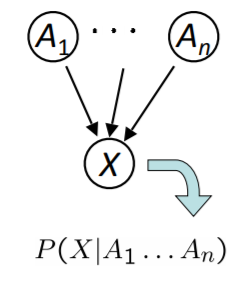
\includegraphics[width=0.25\textwidth]{figs/bayes1.png}
    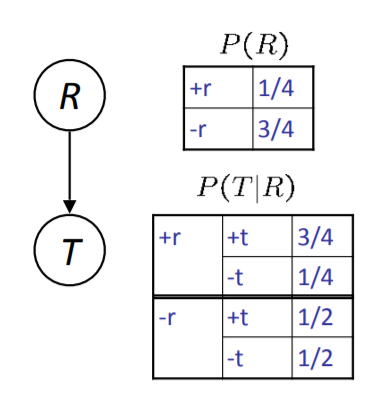
\includegraphics[width=0.25\textwidth]{figs/bayes2.png}
    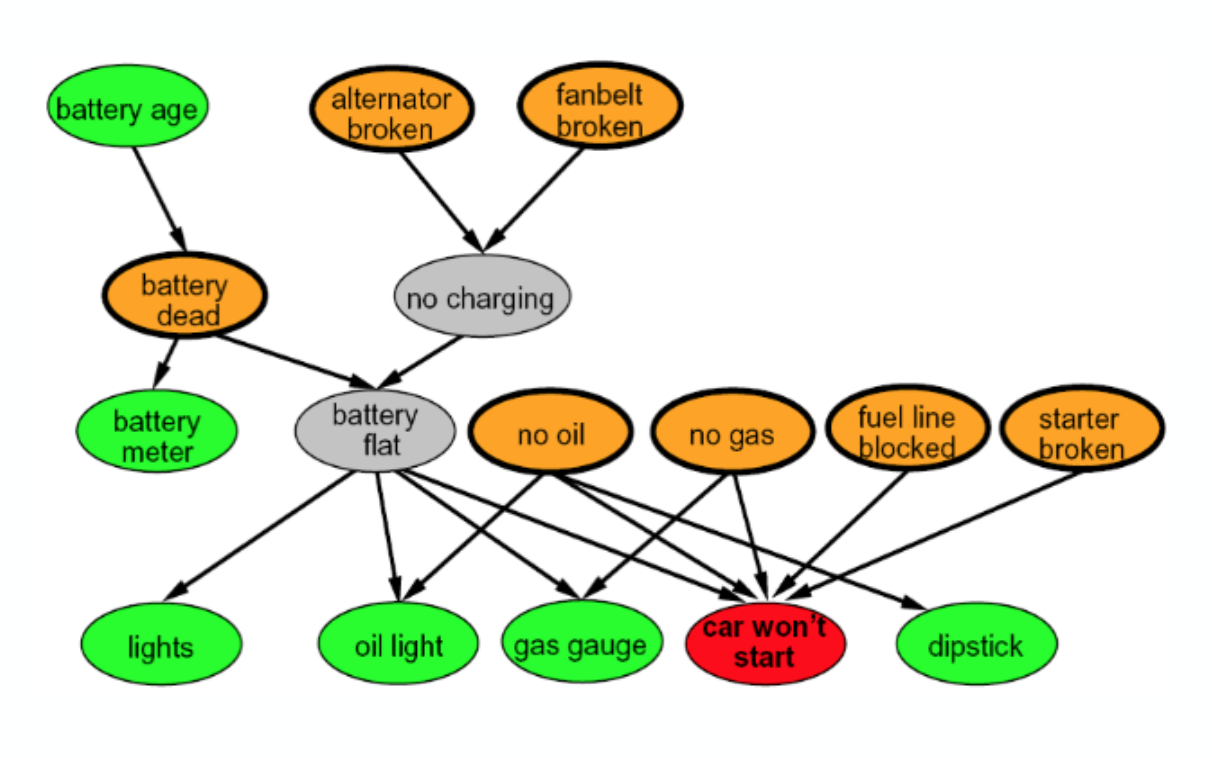
\includegraphics[scale=0.4]{figs/carrepair}
    \caption{Conditional implications example (left), example conditional probability tables (center), and example bayes net for car repair (right)}
    \label{fig:bayes}
\end{figure}

\textbf{Bayes' Nets encode conditional independence.} Just like how the Markov assumption allowed us to simplify equations based on conditional independence across time, the topology of Bayes' Nets can allow us to also assume conditional independence given various pieces of evidence (observed variables). \textbf{D-Separation} is one powerful and simple procedure for determining if $X_i$ and  $X_j$ are conditionally independent given other variables:
\begin{itemize}
    \item Check all undirected paths between $X_i$ and $X_j$
    \item A path is considered active if all triples along it are active and inactive if one or more triples are inactive (and thus breaking the dependence). See Figure~\ref{fig:triples} for the list of active and inactive triples.
    \item If all paths are inactive then we can guarantee conditional independence of $X_i$ and $X_j$. However, if one or more paths are active, then independence not guaranteed.
\end{itemize}

\begin{figure}[ht]
    \centering
    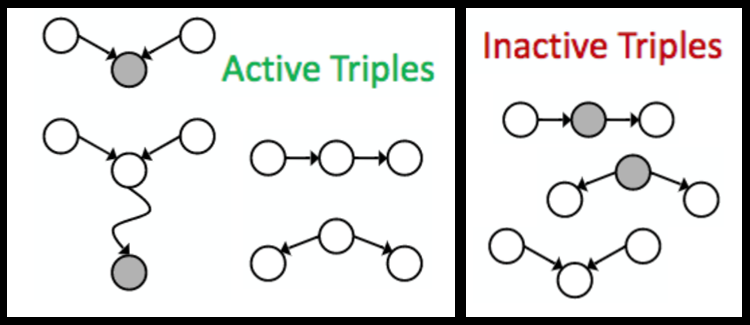
\includegraphics[width=0.6\textwidth]{figs/triples.png}
    \caption{Active and inactive triples for D-Separation. Nodes in grey are assigned. Canonical names for active triples are common effect (left), common cause (bottom right), and causal chain (top right).}
    \label{fig:triples}
\end{figure}

\newpage
\textbf{Inference} is the process of calculating some resulting quantity from a joint distribution (such as a posterior probability $P(X|E_1=e_1,E_2=e_2)$, or most likely explanation $argmax_x \; P(X=x|E_1=e_1,E_2=e_2)$).
\begin{itemize}
    \item \textbf{Enumeration} is the process of creating the full joint distribution over all of the variables and summing out any unneeded variables. For example if you wanted to determine the probability of the variable $Q$ given evidence $E_1=e_1 \ldots E_k = e_k$ but that also related to other variables $H_1 \ldots H_r$ (canonically called ``hidden variables'') you could:
    \begin{enumerate}
        \item Multiply all factors to construct the full joint distribution:
        $$P(Q, H_1, \dots H_r, E_1, \dots, E_k)$$
        \item Sum out all $H_i$ to get joint of query and evidence (selecting rows consistent with the evidence):
        $$P(Q, e_1 \cdots e_k) = \sum_{h_1 \cdots h_r} P(Q, h_1 \cdots h_r, e_1 \cdots e_k)$$
        \item Normalize across all $Q$:
        $$P(Q=q_k | e_1 \cdots e_k) = \frac{P(Q=q_k, e_1 \cdots e_k)}{\sum_{q_i} P(Q=q_i, e_1 \cdots e_k)}$$
    \end{enumerate}
    This proves to be slow as you have to join up the whole joint distribution over all $Q,H,E=e$ before you sum out the hidden variables.
    \item \textbf{Variable Elimination} is a (usually) faster approach (although still NP-Hard) which interleaves joining and marginalizing over the hidden variables. It relies on computing \textbf{factors} which are simply CPTs where some of the variables are observed (selected, known). The process starts with the initial factors, aka the CPTs selecting the known rows just like in enumeration. However instead of forming the full joint distribution we do (see Figure~\ref{fig:enumvselim} for a high level schematic difference):
    \begin{enumerate}
        \item Pick a hidden variable $H_k$
        \item Join all factors mentioning $H_k$ by forming joint distributions:\\
        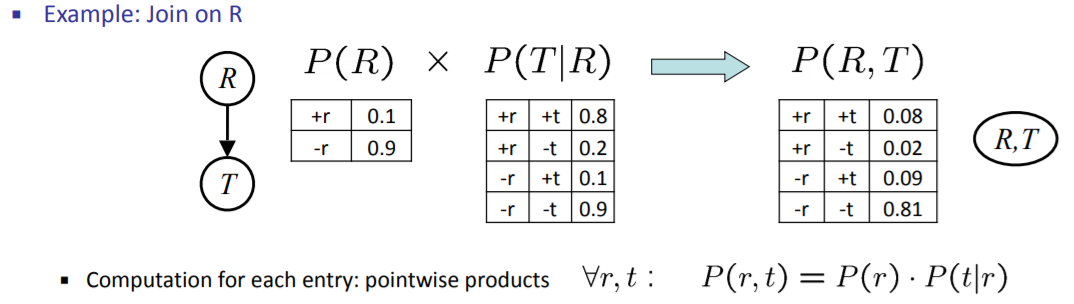
\includegraphics[width=0.8\textwidth]{figs/join.png}
        \item Eliminate (sum out) $H_k$ by computing the marginal distribution:\\
        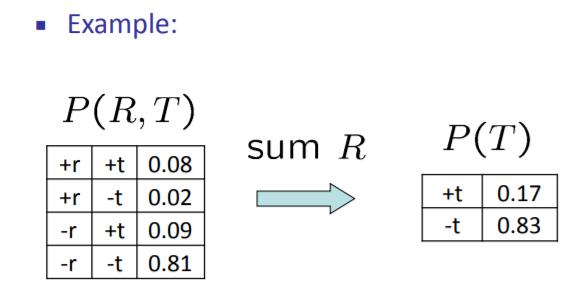
\includegraphics[width=0.4\textwidth]{figs/marginalize.png}
        \item Repeat until all hidden factors are removed. Then do a final join with anything that is left over and normalize!
    \end{enumerate}
    \begin{figure}[ht]
        \centering
        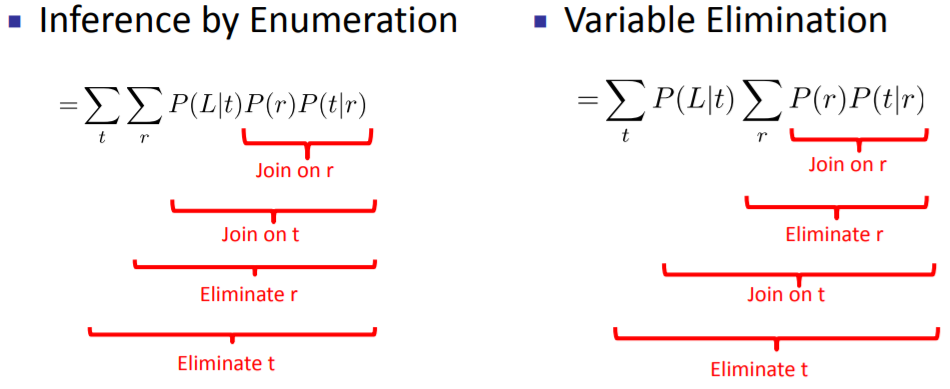
\includegraphics[width=0.6\textwidth]{figs/enumvselim.png}
        \caption{Summary of enumeration vs variable elimination.}
        \label{fig:enumvselim}
    \end{figure}
\end{itemize}

\textbf{Approximate Inference via Sampling}: both Enumeration and Variable Elimination are methods of exact inference (aka you compute the exact answer), but that can be hard as mentioned above. Sampling can be computationally cheaper and provide a very good approximation in many cases (with theoretical guarantees as the number of samples goes to $\infty$). There are a variety of ways to sample:
\begin{itemize}
    \item \textbf{Prior Sampling} is the simplest approach where one simply samples from the CPTs to get a list of samples. Then one can simply use this list to compute approximate probabilities via counting. This is very fast but does not take into account the inference problem we are trying to solve and is simply trying to sample the full joint distribution.
    \item \textbf{Rejection Sampling} modifies Prior Sampling by rejecting any samples that are irrelevant for our inference problem. This allows us to only have to store in memory and compute over the relevent samples. For example if we condition on $E_1 = 0$ (e.g., we are trying to compute $P(Q|E_1 = 0)$) then all samples with $E_1 \neq 0$ can be rejected. Unfortunately, this may reject many many samples.
    \item \textbf{Likelihood Weighting} reduces the number of wasted samples by fixing the evidence variables and then sampling the rest of the distribution. Importantly (to remain consistent) it weights these samples by their likelihood of occurring. Note: evidence only effects ``downstream'' variables from it.
    $$w(Q,E_1 = e_1) = \prod P(e_1 | \text{Parents}(E)) $$
    \item \textbf{Gibbs Sampling} improves Likelihood Weighting by constructing weights that take into account both upstream and downstream evidence through a process known as Markov Chain Monte Carlo (MCMC). You don't need to know this in detail.
\end{itemize}
%%%%%%%%%%%%%%%%%%%%%%%%%%%%%%%%%%%%%%%%%%%%%%%%%%%%%%%%%%%%%%%%%%%%%%%%%
%%%%%%%%%%%%%%%%%%%%%%%%%%%%%%%%%%%%%%%%%%%%%%%%%%%%%%%%%%%%%%%%%%%%%%%%%
\section{Machine Learning}
\noindent Algorithms in machine learning fall under {\bf{supervised}} and {\bf{unsupervised}} approaches. In the former, we are given a set of inputs and labels/outputs, and would like to learn the relationship between them to guess label/output values for new data. In the latter, we are only given input values, and aim to find structure within them.

\subsection{Supervised Learning}
Supervised learning can also be broken down into {\bf{parametric}} and {\bf{non-parametric}} approaches. Parametric algorithms, such as Naive Bayes or regression, rely on learning a set of parameters that define the classifier. Non-parametric algorithms, such as k-NN, rely directly on data rather than on a parameterized model. 

\subsubsection*{Naive Bayes}
Naive Bayes can be thought of as a {\bf{probabilistic inference algorithm}} over a special case of a Bayes Net that is applied to classification. The model is made of an unknown variable $Y$ representing the possible classes, which causes a collection of emission variables $E_1$, $E_2$, $\dots$, $E_n$. We make a (``naive'') assumption that each of the emissions is conditionally independent of one another given $Y$. While this may not be true for most applications, it still results in a simple and useful algorithm. Finally, given the emissions, we can calculate classification probabilities by inference over the Bayes Net:
\[
P(Y | x_1, \ldots, x_n) \propto P(Y, x_1, \ldots, x_n) = P(Y) \prod_{i=1}^n P(x_i|Y)
\]
To build up this network from labeled data, we can count the frequencies of occurrence of observing $(x_i, Y)$ for each $x_i$ and normalize to construct conditional probabilities. Improvements on this approach involve {\bf{smoothing}}, which is discussed further down.

\subsubsection*{Regression}
When the output variable $y$ is continuous rather than discrete, we can perform regression. First, a {\bf{model}} $h_{\theta}$ is chosen to describe the input-output relationship, where the {\bf{model parameters}} $\theta$ are calculated by optimizing over a {\bf{loss function}} $L$ on the training data. For instance, if we assume that the underlying model is {\bf{linear}}, we choose $h_{\theta}(f^{(i)}) = \theta^T f^{(i)}$ for every $i$th data vector. Often, a quadratic loss function is chosen. This is both intuitive, but also theoretically supported -- a quadratic is the {\bf{maximum likelihood estimate}} of the data given the model parameters, under the assumption of i.i.d. Gaussian noise in the data. Overall, the optimization problem to solve {\bf{linear regression}} would be:
\[
\min_{\theta} \; \; \sum_{i = 1}^m (\theta^T f^{(i)} - y^{(i)})^2
\]
There are other possible loss functions, such as:
\begin{itemize}
    \item \bf{absolute ($L_1$) loss}: $L = |h_{\theta}(f) - y|$
    \item \bf{deadband loss}: $L = \max(0, |h_{\theta}(f) - y| - \epsilon)$
\end{itemize}

\noindent {\bf{Logistic regression}} is a variant of regression designed for binary classification (where the output variable does assume discrete values $0$ and $1$). Instead of using the linear function $h_{\theta}(f) = \theta^T f$, we apply a sigmoid:
\[
h_{\theta} = \frac{1}{1 + e^{-\theta^T f}}
\]
Similarly to linear regression, we choose a loss function, pose an optimization problem, and solve for the optimal parameters $\theta$. 

\noindent While linear regression with a quadratic loss is {\bf{convex}} and has a closed-form solution, most of these optimization problems are non-convex and are solved with {\bf{stochastic gradient descent}}. Finally, after an optimization approach is applied and the model parameters $\theta$ are determined, we can guess the output of new data $f$ by calculating $h_{\theta}(f)$ (for the binary logistic case, rounding it to 0 or 1).

\subsubsection*{k-Nearest Neighbors}
This is a simple {\bf{non-parametric}} classification approach which assigns a label to a new point by choosing the most common class of the $k$ closest neighboring points. Variations on this algorithm might give a weighting scheme to the $k$ labels rather than choosing the most common value. 

\noindent When designing an ML algorithm, the available data is usually broken up into the {\bf{training data}}, which is used to train the classifier, and the {\bf{test data}}, which is used to evaluate the classifier and can in no way be viewed or used beforehand. \noindent This division of datasets allows to deal with two issues:
\begin{enumerate}
    \item {\bf{Overfitting}} occurs when a classifier is trained for very high (near 100\%) training accuracy, but is not able to {\bf{generalize}} to the testing data, and has low test accuracy.
    \begin{enumerate}
        \item {\bf{Smoothing}} is used in discrete problems to cause more gradual updates to probabilities. For instance, one example of overfitting would be giving zero probabilities to all words not in the training set, which can be mitigated with {\bf{Laplace smoothing}}:
        \begin{align*}
        &\text{standard probability:} \; \; P_{ML}(x) = \frac{count(x)}{N} \\
        &\text{with smoothing:} \; \; P_{LAP, k}(x) = \frac{count(x) + k}{N + k|X|}
        \end{align*}
        \item {\bf{Regularization}} is used in continuous problems such as regression. For instance, an example of overfitting would be using a high-order polynomial that goes through all training data points. The addition of a regularization term to the loss function places an analytic penalty on problem parameters to encourage smaller values or sparsity:
        \begin{align*}
        &\text{standard loss function:} \; \; loss(f^{(i)}, y^{(i)}, \theta) = (\theta^T f^{(i)} - y^{(i)})^2 \\
        &\text{with $L_2$-regularization:} \; \; loss(f^{(i)}, y^{(i)}, \theta) = (\theta^T f^{(i)} - y^{(i)})^2 + \lambda ||\theta||_2^2 \\
        &\text{with $L_1$-regularization:} \; \; loss(f^{(i)}, y^{(i)}, \theta) = (\theta^T f^{(i)} - y^{(i)})^2 + \lambda ||\theta||_1
        \end{align*}
    \end{enumerate}
    \item Sometimes algorithms depend on a choice of {\bf{hyperparameters}}, which must be decided outside of the training process. There are a couple common approaches to tuning:
    \begin{enumerate}
        \item Part of the training data is taken to be the {\bf{held-out dataset}}. For each hyperparameter value, the classifier is trained with the rest of the training data and tested on the held-out data, and the one with the highest accuracy is chosen.
        \item If there are $m$ possible values for a hyperparameter, {\bf{cross-validation}} divides the training data into $m$ sections. For the $i$th value, the $i$th section is chosen to be the tuning test set and the others are chosen to be the tuning training sets. After evaluating all hyperparameter values, the one with the highest tuning test accuracy is chosen.
    \end{enumerate}
\end{enumerate}


\subsection{Unsupervised Learning}

Unsupervised learning algorithms focus primarily on clustering, dimensionality reduction, anomaly detection, or other ways of inferring data structure without labels. The algorithms we have discussed all fall under clustering.

\noindent {\bf{K-means}} is a {\bf{centroid-based}} clustering algorithm. First, initialize $k$ cluster centroids. Then, iteratively:

\noindent Assign each point to nearest cluster centroid:
\[
a_i = \text{argmin}_k \; \text{dist}(x_i, c_k), \;\; i = 1, \dots, N
\]

\noindent Recompute the $k$th cluster centroid by taking the mean of the points assigned to cluster $k$:
\[
c_k = \frac{1}{|a_i \;:\; a_i = k|} \sum_{(i \;:\; a_i = k)} x_i, \;\; k = 1, \dots, K
\]


\noindent {\bf{Agglomerative clustering}} and {\bf{divisive clustering}} are both {\bf{connectivity-based}} clustering algorithms. The former iteratively constructs larger clusters from smaller clusters. The latter iteratively breaks down large clusters into smaller clusters.

\noindent {\bf{Choosing K:}} The outcome of all of these algorithms vary on the chosen number of clusters. Some common approaches for choosing $k$ are:
\begin{itemize}
    \item We can plot the average of the distances from each point to its cluster's centroid. Then, it is reasonable to choose the smallest value of $k$ for which this ``error'' flattens out.
    \item {\bf{Silhouette diagrams}} are plots of the measure
    \[
    m_i = \frac{(b_i - a_i)}{\max(a_i, b_i)}
    \]
    where $a_i$ is the mean distance from the point $x_i$ to all points in its cluster, and $b_i$ is the mean distance from $y_i$ to all points in the neighboring (``next best'') cluster.
\end{itemize}
%%%%%%%%%%%%%%%%%%%%%%%%%%%%%%%%%%%%%%%%%%%%%%%%%%%%%%%%%%%%%%%%%%%%%%%%%
%%%%%%%%%%%%%%%%%%%%%%%%%%%%%%%%%%%%%%%%%%%%%%%%%%%%%%%%%%%%%%%%%%%%%%%%%
\section{Game Theory}
Game theory studies decision making in systems with multiple, self-interested actors/players and Rewards/payoffs depend on joint actions. In most cases rationality is assumed: a “rational” agent will select an action that maximizes its (expected) payoff. This directly leads to an assumption of selfishness on behalf of both players and therefore, the interaction stabilizes at an equilibrium state where no agent can increase their payoff via unilateral deviation.

In this class we will consider games where we have a set of players ($N = {1, \ldots , n}$), actions ($A = {1, \ldots , m}$), and a utility mapping for each player given the actions of all players ($u_i = A_1 \times \ldots \times A_k \rightarrow R$). One way to solve these types of games is to allow each player to select a \textbf{mixed strategy} $s_i = \{a_1, \dots, a_m \}$ where $a_i$ denotes the probability of choosing action $A_i$ (note: $\sum_i a_i = 1$). Each \textbf{Nash Equilibrium} for a given game occurs when no agents can improve their total utility by changing their strategy. Note that there may be multiple equilibria, that at times a dominant strategy (each play choses a single move with probability 1) may exist, and that the equilibrium outcome is not necessarily the best for players (think prisoners dilemma). While computing Nash Equilibria in general is very hard it can be done relatively easily for two player zero sum games (which is all that you need to know for this exam).

To solve two player zero sum games we want to write our game, $G = (N,A,u)$, in \textbf{Normal Form}: a matrix where each row (and column) represent the action taken by the row (and column) player and where each cell is a tuple specifying the utilities for the (row, column) players. The solution according to Von Neumann’s theorem (which we proved in class) is a mixed strategy where we solve the maximin problem (essentially minimax with depth 2).
$$ s_1^* = max_{s_1} min_{a_2} u_1(s_1, a_2)$$
For example consider the "matching pennies" problem shown below:\\
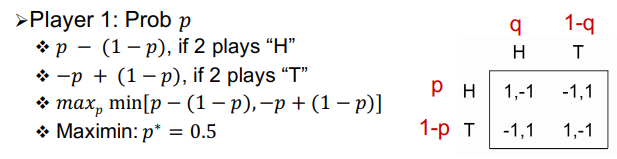
\includegraphics[width=0.5\textwidth]{figs/matchingPennies.png}\\
Where we note that the solution to the maximin problem is to set the two equations equal to each other as the only way the choice of $p$ can both maximize and minimize the utility is if the utility is equal in each state. The same argument would hold for more than 2 moves but it would require solving a system of equations. Note that if there are an unequal number of moves for the two players this system of equations approach will be under-determined for the player with more moves and further inspection will be required to find the solution that maximizes utility for that player while satisifing the under-determined system.
\end{document}
